%#!pdflatex Naruse_Esurf_2020.tex

\section{Forward model description}

Here we describe the formulation of the forward model used for producing training datasets for the inverse model (Fig. \ref{fig:model_explanation}). This model is based on the model developed by \citet{kostic2006response}, which predicts the behavior of surge-type turbidity currents, but we modified it to consider sediment transport and deposition of multiple grain-size classes. The initial setting of the flows was set to be the lock-exchange condition, which assumes that the collapse of a rectangular-shaped cloud of sediment suspension produces a turbidity current.

\begin{figure*}[t]
  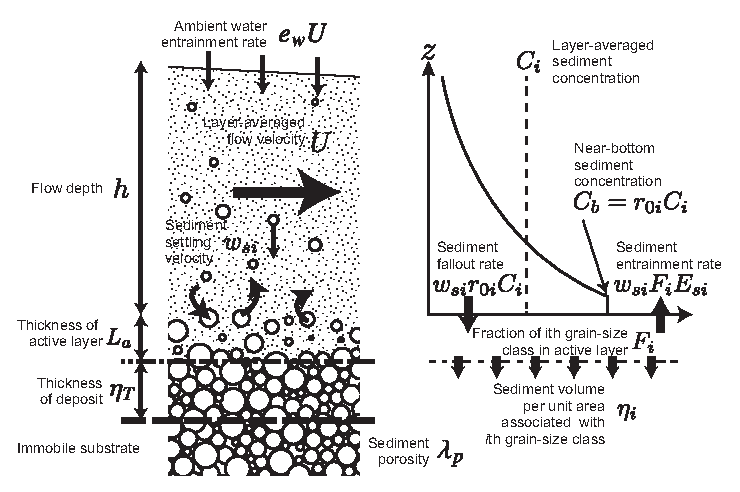
\includegraphics[width=12cm]{fig02.eps}
  \caption{Explanation of model parameters. The turbidity current exchanges suspended sediment with the active layer ($L_{a}$ in thickness) on the top of the deposit ($\eta_T$ in thickness) by settling and entrainment. The volumetric rate of settling of the $i$th grain-size class of sediment is calculated from the basal sediment concentration $r_{0} C_i$ multiplied by the sediment settling velocity $w_{s}{i}$. The sediment entrainment rate from the active layer is $w_{si} F_i e_{si}$, where $F_i$ is the volumetric fraction of the $i$th grain-size class in the active layer and $E_{si}$ is the unit dimensionless rate of sediment entrainment. The time variation of grain-size distribution in the active layer is computed in this model.}
  \label{fig:model_explanation}
\end{figure*}


\subsection{Layer-averaged equations}

Let $t$ and $x$ be the time and bed-attached streamwise coordinates, respectively. Parameters $U$ and $h$ denote the layer-averaged flow velocity and the depth, respectively. The total sediment concentration is $C_T$. Here, we apply the following layer averaged conservation equations of fluid mass, momentum and suspended sediment mass of a turbidity current \citep{parker1986self,kostic2006response}:

\begin{eqnarray}
  \frac{\partial h}{\partial t} + \frac{\partial Uh}{\partial x} & = & e_wU \label{eq:conserv_fluidmass} \\
  \frac{\partial Uh}{\partial t} + \frac{\partial U^2h}{\partial x} & = & R g C_T h S - \frac{Rg}{2}\frac{\partial C_T h^2}{\partial x} - C_f U^{2} \label{eq:conserv_momentum} \\
\frac{\partial C_i h}{\partial t} + \frac{\partial U C_i h}{\partial x} & = & w_{si} (F_i e_{si} - r_0 C_i) \label{eq:conserv_suspensionmass}
\end{eqnarray}

\noindent where $R(=\rho_s/\rho_f - 1)$ is the submerged specific density of the sediment ($\rho_s$ and $\rho_f$ are the densities of the sediment and the fluid), and $g$ is the gravity acceleration. $S$ is the slope, and $C_f$ denotes the friction coefficient. The right-hand side of the fluid mass conservation (Equation \ref{eq:conserv_fluidmass}) considers the entrainment of ambient fluid to the flow, in which the empirical entrainment coefficient $e_w$ is applied. Equation \ref{eq:conserv_suspensionmass} describes the mass conservation of the suspended sediment in the flow, which varies depending on the balance between settling and entrainment of the sediment from and to the active layer. In this model, the grain-size distribution of sediment is discretized to $N$ classes. The parameter $C_i$ denotes the suspended sediment concentration of the $i$th class. The model applies the active layer assumption, in which the grain-size distribution is vertically uniform in the bed surface layer (active layer) that exchanges sediment with suspended load \citep{Hirano1971}. $F_i$ indicates the fraction of the $i$th grain-size class in the active layer. The parameter $w_{si}$ denotes the settling velocity of the sediment particles in the $i$th class, and $r_0$ denotes the ratio of near-bed concentration to the layer-averaged concentration of the suspended sediment.

The mass conservation of the sediment in the active layer and the deposit (historical layer), respectively, takes respectively the form

\begin{eqnarray}
  \frac{\partial \eta_i}{\partial t} & = & \frac{w_{si}}{1-\lambda_p}(r_0 C_i - e_{si} F_i) \label{eq:conserv_bed} \\
\frac{\partial \eta_T}{\partial t} &=& \sum \frac{\partial \eta_i}{\partial t}.
\label{eq:total_exner_equation} \\
\frac{\partial F_i}{\partial t} + \frac{F_i}{L_a}\frac{\partial \eta_T}{\partial t} & = & \frac{w_{si}}{L_a (1 - \lambda_p)}(r_0 C_i - F_i e_{si} ). \label{eq:conserv_activelayer}
\end{eqnarray}

\noindent where $\eta_i$ denotes the volume per unit area of the $i$th grain size class, and $\eta_T$ is the total thickness of the deposit. $L_a$ denotes the thickness of the active layer, which is assumed to be constant, for simplicity. The parameter $\lambda_p$ denotes porosity of the active layer and the deposit (0.4 in this study), and $e_{si}$ is an empirical coefficient for sediment entrainment of the $i$th class from the active layer. Equation \ref{eq:conserv_bed} describes the mass conservation of the $i$th class sediment in the bed, and rate of the bed aggradation is obtained by summation of accumulation rates of all grain-size classes (Equation \ref{eq:total_exner_equation}). Equation \ref{eq:conserv_activelayer} considers the temporal development of the grain size distribution in the active layer, where the time development of the total bed thickness $\eta_T$ is obtained by summation of the right-hand side of Equation \ref{eq:conserv_bed} for all grain-size classes.

To solve the Equations \ref{eq:conserv_fluidmass}--\ref{eq:conserv_activelayer}, empirical relations are required for the parameters: $w_{si}$, $r_0$, $C_f$, $L_a$, $e_w$, and $e_{si}$. Here we applied the formulation of \citet{dietrich1982settling} for obtaining the settling velocity $w_{si}$. The ratio of near-bed to layer-averaged concentrations $r_0$ and the bed friction coefficient $C_f$ are fixed to be 2.0 and 0.004, for simplicity \citep{Garcia1990}. The active layer thickness $L_a$ is assumed to be constant (0.003 m). Regarding the entrainment coefficients of ambient water and basal sediment $e_w$ and $e_{si}$, we applied formulations proposed by \citet{parker1987experiments} and \citet{garcia1991entrainment} respectively.

For computational efficiency and numerical stability, a deformed grid approach was adopted to solve Equations \ref{eq:conserv_fluidmass}--\ref{eq:conserv_suspensionmass}. In this transformed coordinate, the propagating flow head was fixed at the downstream boundary using a Landau transformation \citep{Crank1984}. The tail of the flow was also fixed at the upstream end of the calculation domain, and thus the grid spacing in the dimensional coordinate space was continuously stretched during calculation, whereas that in dimensionless space remained constant. This scheme was based on \citet{kostic2006response}, and more details regarding the numerical implementation were given by \citet{Nakao2017}.

\subsection{Model input parameters and topographic settings}
In this study, a turbidity current was assumed to occur from a cloud of suspended sediment (height: $H_0$, length $l_0$). The initial flow velocity was set to 0, and the sediment of the $i$th grain-size class was considered to be initially homogeneously distributed in the suspension cloud at the concentration $C_i$ (Fig. \ref{fig:model_input_parameters}). The suspended sediment cloud was located at the upstream end of the calculation domain, where the slope gradient was 0.1. This steep slope extended for 5.0 km and transited to a gently sloping basin plain (gradient is $S_l$) in the downstream region. Total length of calculation domain was 100 km. In summary, the number of initial conditions required for the forward model calculation was three ($H_0$, $l_0$ and $S_l$) plus number of grain-size classes ($C_i$). 

\begin{figure}[t]
  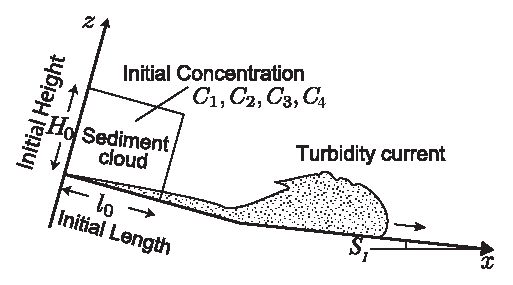
\includegraphics[width=8.3cm]{fig03.eps}
  \caption{Model input parameters. The initial conditions of turbidity current is assumed to be the suspended sediment cloud that is $H_0$ and $l_0$ in height and length, respectively. The initial sediment concentrations $C_1$ to $C_4$ and the basin slope $S_l$ are to be specified for calculation. These seven input parameters are subject to be reconstructed by inverse analysis.}
  \label{fig:model_input_parameters}
\end{figure}
